\section{Neudefinition des Verhaltens von interaktiven Karten} \label{sec:analyse-karten}

Die interaktiven Karten der App erwiesen sich in den Benutzertests als sehr enttäuschend und kaum nutzbar (siehe \ref{sec:user_tests_results}).
Es ist notwendig, neu zu überdenken, was die Nutzer von einer solchen Karte erwarten, um die für sie relevantesten Features anbieten zu können.
Dieser Teil wird sich auf die Ideation der zu implementierenden Features, die Darstellung der Gruppierung von Punkten in verschiedenen Clustern und die Auswahl der UI konzentrieren, die es ermöglicht, \textit{Sites} und ihre Sensoren mit ihrem jeweiligen Status geografisch zu repräsentieren.

\subsection{Ideation im Team}

Bei einer solch niedrigen Usability-Punktzahl ist es von entscheidender Bedeutung, die Ziele der interaktiven Karten, mit denen eine \textit{Site} angezeigt wird, neu zu bewerten.
Dazu wurde eine schnelle Brainstorming-Sitzung mit dem Cloud-Team durchgeführt.
Das Thema der Reflexion lautete: \textit{Was sollte auf der interaktiven Kartenseite möglich sein?}.
Der Fortschritt der Überlegungen zum Miro-Tool kann im Anhang \ref{appendix:question_board_map} nachgelesen werden, der sich in den folgenden Bedürfnissen zusammenfassen lässt:

\begin{table}[H]
  \begin{tabular}{p{0.3\linewidth} |p{0.7\linewidth}}
    Konzept                                               & Beschreibung                                                                                                                                                                                                                                                                                                                                                                        \\ \hline\hline

    \textbf{Darstellung von \textit{Sites} und Apparaten} & Die Karte muss in der Lage sein, Sensoren und \textit{Sites} auf intuitive Weise darzustellen. Das bedeutet, dass der Nutzer jeden Sensor, jedes \textit{Borders-Gateways} und jedes \textit{Mesh-Gateways} einzeln erkunden kann. Dasselbe gilt für \textit{Sites}, wo er in der Lage sein sollte, jeden \textit{Site} und alle Geräte, die ihn bilden, einzeln zu identifizieren. \\\hline
    \textbf{Clustering von Aufmerksamkeitspunkten}        & Die \textit{Sites} und verschiedenen Geräte sollten auf jeder Zoomstufe der interaktiven Karte sichtbar und leicht identifizierbar sein. Das bedeutet, dass die einzelnen Punkte nicht überlappen, sondern zusammengefasst werden sollten, um eine überfüllte Karte zu vermeiden.                                                                                                   \\\hline
    \textbf{Anzeige der Sensorstatue}                     & Die einzelnen Sensoren können verschiedene Status haben, z. B. dass sie stabil sind, dass der Batteriestand zu niedrig ist oder dass sie einen Waldbrand erkennen. Es sollte möglich sein, jeden dieser Status für jedes Gerät auf jeder Zoomstufe der Karte zu identifizieren.
  \end{tabular}
  \caption{Konzepte, die in die interaktive Karte implementiert werden sollen}
\end{table}

\subsection{Clustering von Sensoren und \textit{Sites}}

Die aktuelle Karte implementiert kein Clusturing-System.
Stattdessen wird auf der Google-Map ein bläulicher Kreis angezeigt, dessen Größe relativ zu den Sensoren ist.
Wenn der Benutzer auf ein vordefiniertes Level zoomt, wird eine \ac{HTTP}-Anfrage gesendet, um die Standorte aller Sensoren in allen Listen abzurufen und sie auf der Karte anzuzeigen.
Diese naive Implementierung wurde eingeführt, um zu vermeiden, dass alle Marker der verschiedenen Sensoren direkt angezeigt werden, was die Karte unleserlich machen würde.
Das führt zu einem schrecklichen Erlebnis, bei dem der Nutzer, wenn er zu weit herauszoomt, die \textit{Sites} nicht sieht, weil sie zu klein sind, und wenn er zu weit hineinzoomt, fragt er sich, wo die Sensoren sind, weil die Suche sehr langsam ist, da sie alle Sensoren von allen \textit{Sites} zurücksendet.

Es gibt jedoch ein Konzept für die Interaktion von Punkten, das in den meisten Produkten zur Implementierung interaktiver Karten verwendet wird und seine Effektivität unter Beweis stellt: Clustering.
Die Idee dahinter ist sehr einfach: Wenn sich zwei oder mehr Punkte beim Zoomen überlappen, werden sie in einem neuen Punktdesign zusammengefasst, um die Anzahl der eingeschlossenen Punkte zu schätzen.
Auf die gleiche Weise werden beim Zoomen die nicht mehr überlappenden Punkte aus dem Cluster herausgeschleudert und wieder zu Originalpunkten.

// TODO

\begin{figure}[H]
  \centering
  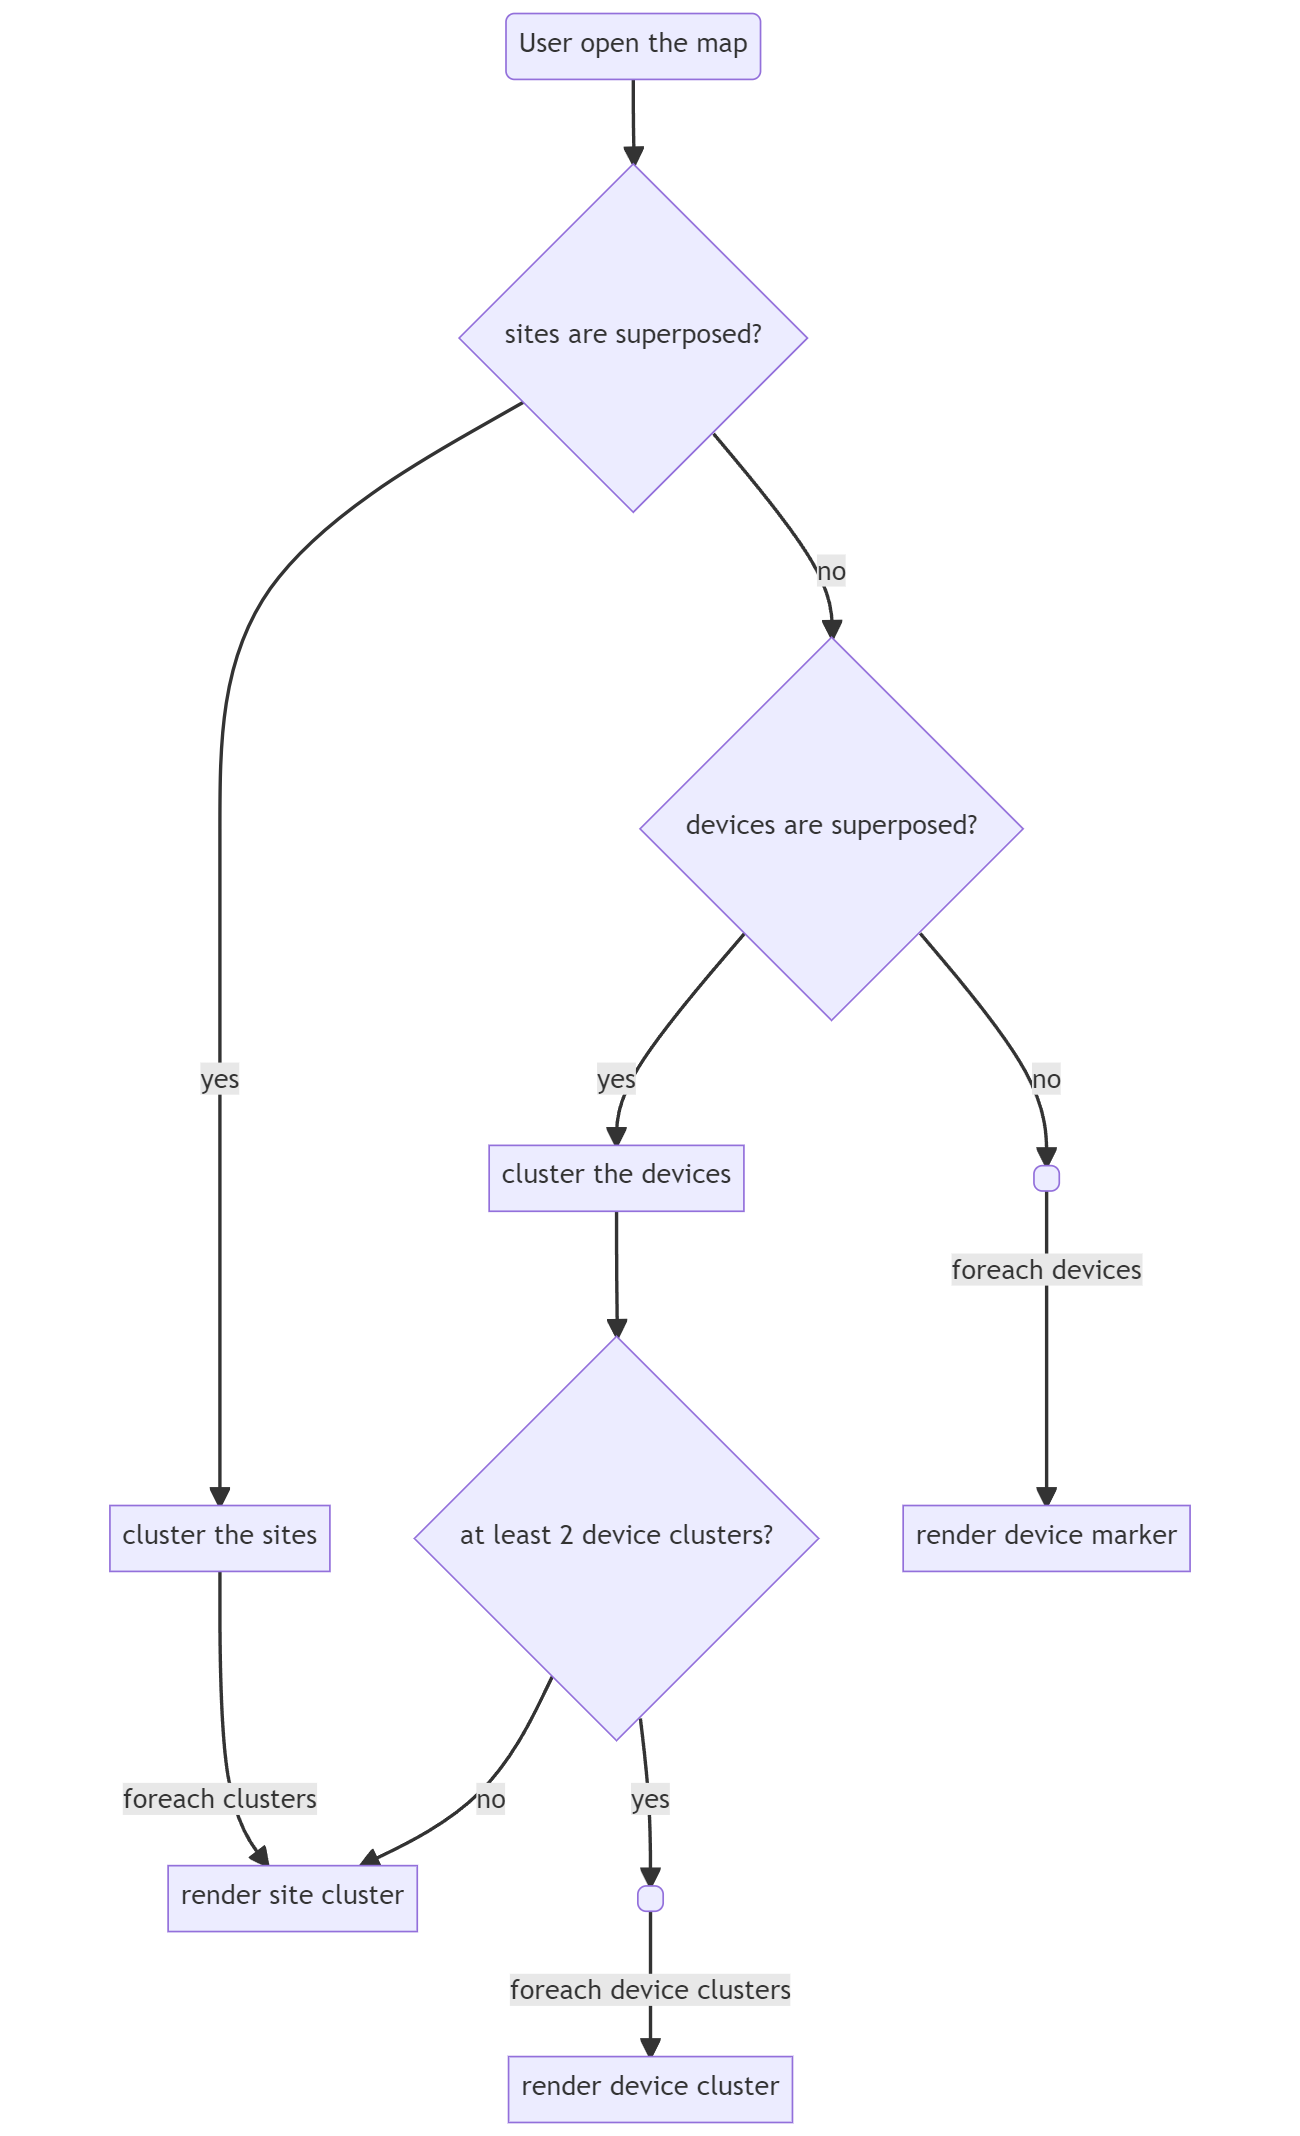
\includegraphics[width=13cm]{map_clustering_flow}
  \caption{}
  \label{fig:map_clustering_flow}
\end{figure}
